% standalone document border convention: {left bottom right top}
\documentclass[varwidth=267pt,border={0pt, 0pt, 1pt, -9pt}]{standalone}
\usepackage[force]{feynmp-auto}		    
\usepackage{amsmath}
\usepackage{graphicx}

\begin{document}
\begin{flalign*}
	\Gamma^{(4)}_{1234} &\hspace*{0.5ex}=\hspace*{0.5ex}
	\delta_{13}\delta_{24}
	\left(\hspace*{0.25ex}
	\scalebox{0.75}{$
			\begin{gathered}
				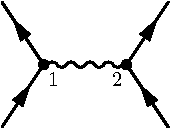
\includegraphics{gamma4/gamma4_1a.pdf}
			\end{gathered}
		$}
	\hspace*{0.5ex}+\hspace*{0.5ex}
	\scalebox{0.75}{$
			\begin{gathered}
				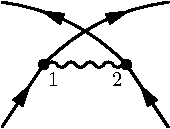
\includegraphics{gamma4/gamma4_1b.pdf}
			\end{gathered}
		$}
	\hspace*{0.25ex}\right)
	\\
	&\hspace*{3ex}+\hspace*{0.5ex}
	\delta_{13}\delta_{24}
	\left(\hspace*{0.25ex}
	\scalebox{0.75}{$
			\begin{gathered}
				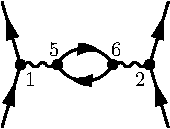
\includegraphics{gamma4/gamma4_2a.pdf}
			\end{gathered}
		$}
	\hspace*{0.5ex}+\hspace*{0.5ex}
	\scalebox{0.75}{$
			\begin{gathered}
				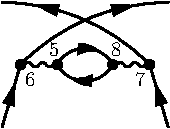
\includegraphics{gamma4/gamma4_2b.pdf}
			\end{gathered}
		$}
	\hspace*{0.25ex}\right)
	\hspace*{0.5ex}+\hspace*{0.5ex} \cdots
\end{flalign*}
\end{document}

&